\documentclass[tikz,border=4pt]{standalone}
\usepackage{amsmath,amssymb}
\usetikzlibrary{arrows.meta,calc,decorations.pathreplacing}
\definecolor{cA}{HTML}{924800}
\definecolor{cB}{HTML}{2F7FC8}
\definecolor{cC}{HTML}{39994B}
\tikzset{
  pt/.style={circle,fill=black,inner sep=0pt,minimum size=4pt},
  disp/.style={-{Stealth[length=2.6mm,width=2mm]},line width=0.9pt,shorten <=2.5pt,shorten >=2.5pt},
  lab/.style={font=\small,sloped,text=black},
  brc/.style={decorate,decoration={brace,amplitude=5pt,raise=3pt},line width=0.6pt},
}
\begin{document}
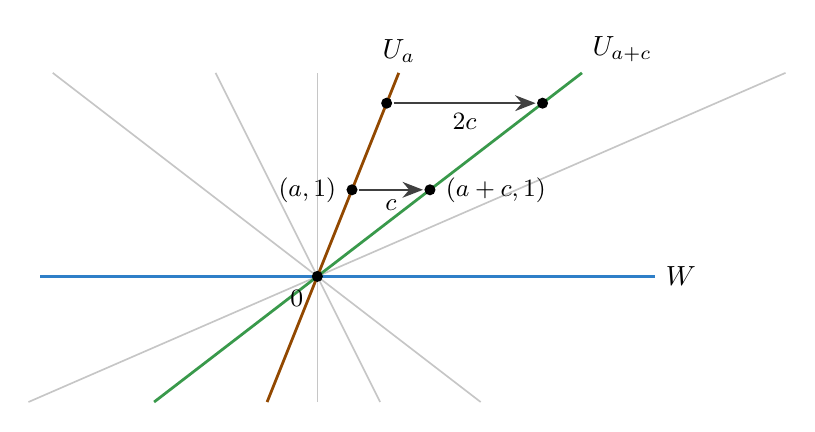
\begin{tikzpicture}[scale=1.1]
  \def\a{0.4} \def\c{0.9}
  % other complements
  \foreach \s in {-1.3,-0.5,0,2.3}
    \draw[gray!45,line width=0.6pt] ({-1.45*\s},-1.45) -- ({2.35*\s},2.35);
  % W
  \draw[cB,line width=1.1pt] (-3.2,0) -- (3.9,0) node[right,text=black]{$W$};
  % highlighted complements
  \draw[cA,line width=1pt] ({-1.45*\a},-1.45) -- ({2.35*\a},2.35) node[above,text=black]{$U_a$};
  \pgfmathsetmacro{\ac}{\a+\c}
  \draw[cC,line width=1pt] ({-1.45*\ac},-1.45) -- ({2.35*\ac},2.35) node[above right,text=black]{$U_{a+c}$};
  % shear arrows at heights 1 and 2
  \draw[disp,black!75] (\a,1) -- node[lab,below]{$c$} (\ac,1);
  \draw[disp,black!75] ({2*\a},2) -- node[lab,below]{$2c$} ({2*\ac},2);
  \node[pt,label={[font=\small]left:$(a,1)$}] at (\a,1) {};
  \node[pt,label={[font=\small]right:$(a+c,1)$}] at (\ac,1) {};
  \node[pt] at ({2*\a},2) {}; \node[pt] at ({2*\ac},2) {};
  \node[pt,label={[font=\small]below left:$0$}] at (0,0) {};
\end{tikzpicture}
\end{document}
